%!TEX root = paper.tex
\chapter{InferSpark Overview}
\label{chap:framework}
\begin{figure*}[!ht]
	\centering
    \includegraphics[width=0.9\linewidth, clip]{figs/workflow_future.eps}
    \caption{InferSpark architecture}
    \label{fig:workflow}
\end{figure*}

The overall architecture of InferSpark is shown in \figref{fig:workflow}.  An
InferSpark program is a mix of Bayesian network model definition and ordinary 
user code. The Bayesian network construction module separates the model part
out, and transforms it into a Bayesian network template. The algorithm
matching module selects the applicable inference algorithm (e.g. variational
message passing). The template is
then instantiated with parameters and metadata from the input data at run time
by the code generation module, which produces the inference code. These are
then executed on the Spark distributed engine to produce the final posterior
distribution.

Next, we describe the key modules in more details with the example of the
two-coin model (\figref{fig:two_coin_bn}). 

\section{Running Example}

\begin{figure}[h]
\begin{lstlisting}
@Model class TwoCoins(alpha: Double, beta: Double) {
	val pi = Beta(alpha)
	val phi = (0L until 2L).map(_ => Beta(beta))
	val z = ?.map(_ => Categorical(pi))
	val x = z.map(z => Categorical(phi(z)))
}
object Main {
	def main() {
		val xdata: RDD[Long] = /* load (observed) data */
		val m = new TwoCoins(1.0, 1.0)
		m.x.observe(xdata)
		m.infer(steps=20)
		val postPhi: VertexRDD[BetaResult] = m.phi.getResult()
		/* postprocess */
		...
	}
}
\end{lstlisting}
\caption{Definition of two-coin model in InferSpark}
\label{fig:two_coins_modeldef}
\centering
\end{figure}

\figref{fig:two_coins_modeldef} shows the definition of the two-coin model in
InferSpark (lines 1 - 6) and the user program (lines 7 - 17) that invokes the
inference API. The definition starts with the ``{\sf @Model}'' annotation.  The
rest is similar to a class definition in Scala. The model parameters (``{\sf
alpha}'' and ``{\sf beta}'') are constants to the model. In the model body,
only a sequence of value definitions are allowed, which define random
variables instead of ordinary deterministic variables.  The use of ``{\sf val}''
instead of ``{\sf var}'' in the syntax implies the conditional dependencies
between random variables are fixed once defined. For example, line 2 defines
the random variable $\pi$ having a symmetric Beta prior $\mathrm{Beta}(\alpha,
\alpha)$.

InferSpark model uses ``Range'' class in Scala to represent plates. Line 3
defines a plate of size 2 with the probabilities of seeing head in the two
coins. Line 4 defines a plate of indexes of the chosen coins. The ``?'' is a
special type of ``Range'' representing a plate of unknown size at the time of
model definition.  In this case, the exact size of the plate will be provided
or inferred from observed variables at run time.  When a random variable is
defined by mapping from a plate of other random variables, the new random
variable is in the same plate as the others.  For example, line 5 defines the
outcomes $x$ as the mapping from $z$ to Categorical mixtures, therefore $x$
will be in the same plate as $z$. Since the size of the plate surrounding $x$
and $z$ is unknown, we need to specify the size at run time.  We can either
explicitly set the length of the ``?'' or let InferSpark set that based on the
number of observed outcomes $x$ (line 11).

At the first glance, ``?'' seems redundant since it can be replaced by a
model parameter $N$ denoting the size of the plate.  However, ``?'' becomes
more useful when there are nested plates. In the two-coin model, suppose
after we choose one coin, we toss it multiple times. 
\figref{fig:two_coins_nestedplates} shows this scenario.
Then the outcomes $x$ are in two nested plates where the inner plate is
repeated $M$ times, and each instance may have
a different size $N_i$. Using the ``?'' syntax
for the inner plate, we simply change line 5 to
\begin{center}
\begin{verbatim}
	val x = z.map(z => ?.map(_ => Categorical(phi(z))))	
\end{verbatim}
\end{center}

\begin{figure}[th]
	\centering
	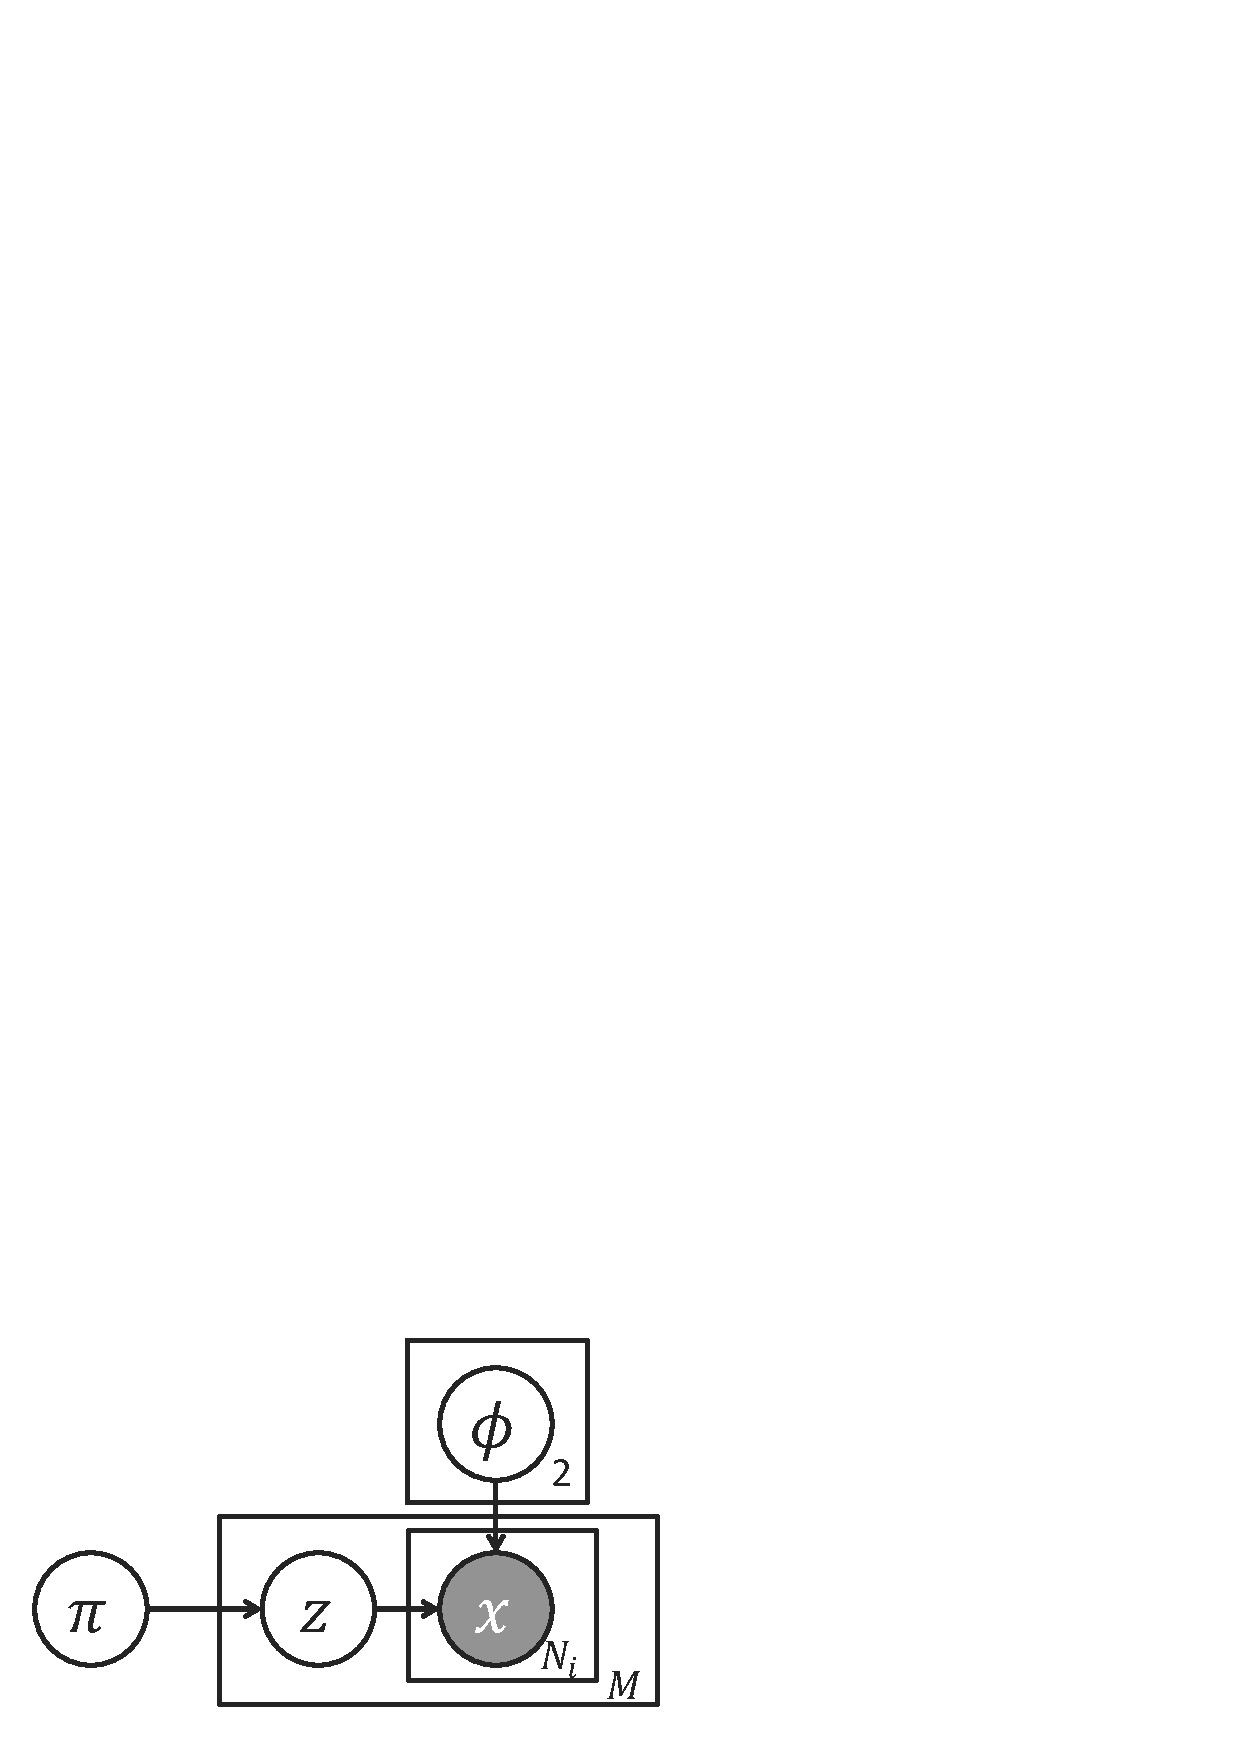
\includegraphics[scale=0.5, clip]{figs/two_coins_nestedplates}
	\caption{Two-coin model with nested plates}
	\label{fig:two_coins_nestedplates}
\end{figure}

\section{Bayesian Network Construction}

\begin{figure}[h]
\centering
\includegraphics[scale=0.5,clip]{figs/two_coins_bn1.eps}
\caption{Bayesian network template constructed from the two-coin model}
\label{fig:two_coins_bn1}
\end{figure}

An input InferSpark program is first parsed and separated into two parts: 
the model definition (``{\sf @Model} class TwoCoins'' in 
\figref{fig:two_coins_modeldef}) and
the ordinary scala program (``{\sf object Main}'' in
\figref{fig:two_coins_modeldef}). The model definition is analyzed and
transformed into valid scala classes that define a Bayesian
network constructed from the model definition 
(e.g., \figref{fig:two_coins_bn1}) and the inference/query API.
Note the Bayesian network
constructed at this stage is only a template (different than 
\figref{fig:two_coin_bn}) because some of the information is not available 
until run time (e.g., the outcomes $x$, the number of coin flips 
and the model parameters $\alpha$ and $\beta$). 

\section{Metadata Collection}

Metadata such as the observed variables and the plate sizes missing from the
Bayesian networks are collected at run time. In the two-coin
model, an instance of the model is created via the constructor invocation (e.g.
``{\sf val m = new TwoCoin(1.0, 1.0)}'' on line 10 of \figref{fig:two_coins_modeldef}). The constructor call provides
the missing constants in the prior distributions of $\pi$ and $\phi$. 
For each random variable defined in the model definition, 
there is an interface field with the
same name in the constructed object. Observed values are provided to InferSpark
by calling the ``{\sf observe}'' (line 11 of \figref{fig:two_coins_modeldef}) 
API on the field. 
There, the user provides an RDD of observed outcomes ``{\sf xdata}'' to InferSpark by calling
``{\sf m.x.observe(xdata)}''. The  {\sf observe} API also triggers 
the calculation of unknown plate sizes. 
In this case, the size of plate surrounding $z$ and $x$ is
automatically calculated by counting the number of elements in the RDD.

\section{Algorithm Matching \& Code Generation}

\begin{figure}[h]
\centering
	\includegraphics[width=0.5\textwidth]{figs/two_coins_msg.eps}
	\caption{Bayesian network with messages for two-coin model}
	\label{fig:two_coins_msg}
\end{figure}

When the user calls ``{\sf infer}'' API (line 12 of
\figref{fig:two_coins_modeldef}) on the model instance, InferSpark checks
whether all the missing metadata are collected. If so, it proceeds to
algorithm matching module. In this case, the module finds that the model is in
exponential-conjugate family so the VMP algorithm is applicable to it. The
Code Generation module then annotates the Bayesian network with the messages used
in VMP, resulting in \figref{fig:two_coins_msg}. The expressions that
calculate the messages (e.g., $E_{Q_\pi}[\ln \pi]$) depend on not only the
structure of the Bayesian network and whether the vertices are observed or
not, but also practical consideration of efficiency and constraints on GraphX and Spark.

To convert the Bayesian network to a message passing graph on GraphX,
InferSpark needs to construct a VertexRDD and an EdgeRDD. This step generates
the MPG construction code specific to the data.
\figref{fig:two_coins_mpg_constr_code} shows the MPG construction code
generated for the two-coin model. 
The vertices are constructed by the union
of three RDD's, one of which from the data and the others from 
parallelized collections (lines 8 and 9 in \figref{fig:two_coins_mpg_constr_code}).
The edges are built from the data only. 
A partition strategy specific to the
data is also generated in this step.


\begin{figure}[h]
\centering
\begin{lstlisting}
class TwoCoinsPS extends PartitionStrategy {
	override def getPartition /**/
}
def constrMPG() = {
	val v1 = Categorical$13$observedValue.mapPartitions{
		initialize z, x */
	}
	val v2 = sc.parallelize(0 until 2).map{ /* initialize phi */ }
	val v3 = sc.parallelize(0 until 1).map{ /* initialize pi */ }
	val e1 = Categorical$13$observedValue.mapParititons{
		/* initialize edges */
	}
	Graph(v1 ++ v2 ++ v3, e1).partitionBy(new TwoCoinsPS())
}
\end{lstlisting}
\caption{Generated MPG construction code}
\label{fig:two_coins_mpg_constr_code}
\end{figure}

In addition to generating code to build the large message passing graph,
the CodeGen module also generates code for VMP iterative inference. 
InferSpark, which
distributes the computation, needs to create a schedule of parallel updates
that is equivalent to the original VMP algorithm, which only updates one vertex
in each iteration. Different instances of the same random variables can be
updated at the same time. An example update schedule for the two-coins model is
($\pi$ and $\phi$) $\rightarrow$ $x$ $\rightarrow$ $z$ $\rightarrow$ $x$. VMP inference code that enforces the update
schedule is then generated. % \ERIC{how to derive this indeed?}

InferSpark currently include the VMP algorithm while other inference
algorithms such as Belief Propagation, Gibbs Sampling and etc. will be added
to it in order to support inference on a wider range of Bayesian networks. We
will also publish a high-level language for implementing inference algorithms
and specifying what models the algorithms apply to.  Algorithm developers are
welcomed to add new algorithms whenever existing ones do not fit the needs of
end-users. Algorithm matching module searches for an applicable algorithm
among both the built-in and the developer-supplied inference algorithms while
the new CodeGen module transforms the algorithm into a Spark program and
handles all the low-level optimization. These two modules are similar to
efforts like SystemML, MLI, which targets algorithm developers, but the two
modules are integrated parts of InferSpark.

\section{Getting the Results}
The inference results can be queried through the ``{\sf getResult}''
API on fields in the model instance. The method retrieves a VertexRDD of approximate
marginal posterior distribution of the corresponding random variable. For
example, in Line 13 of \figref{fig:two_coins_modeldef}, ``{\sf m.phi.getResult()}'' 
returns a VertexRDD of two Dirichlet distributions. 
The user can also call ``{\sf lowerBound}'' 
on the model instance to get the evidence lower bound (ELBO) of the result, 
which is higher when the KL divergence between the approximate posterior 
distribution and the true posterior is smaller. 

\begin{figure}[h]
\centering
\begin{lstlisting}
var lastL: Double = 0
m.infer(20, { m =>
	if ((m.roundNo > 1) || 
		(Math.abs(m.lowerBound - lastL) < 
		   Math.abs(0.001 * lastL))) {
		false
	} else {
		lastL = m.lowerBound
		true	
	}
})
\end{lstlisting}
\caption{Using callback function in ``infer'' API}
\label{fig:two_coins_callback}
\end{figure}

The user can also provide a callback function that will be called after
initialization and each iteration. In the function, the user can write code to
implement customized termination criterion based on the inference result so
far.  For example, this function may return {\em false} whenever the ELBO
improvement is smaller than a threshold (see \figref{fig:two_coins_callback})
indicating the result is good enough and the inference should be terminated. 

